\chapter{Motion in a Circle}
\section{Radians and Degrees}
To discuss circular motion we need to know how to describe angles, eg how round in a circle we have gone. Often when working with circles we do not describe angles in terms of degrees but instead use units called radians.  You are likely to be familiar with describing angles in a degrees where a full rotation is $360^{\circ}$ and a half rotation is $180^{\circ}$. \textbf{Radians} are an alternative, and some would say ``better'' method of measuring angles, the certainly simplify some computations, though they can seem confusing when we first meet them.\\

The basic idea of radians is to work in terms of the distance around the circle that the angle corresponds to.  For a circle with radius $r$ the circumference is $c=2\uppi r$, while an arc of the circle would have length s, shown in red in \cref{fig: radians}. Radians are defined in terms of the length of arcs as
\begin{equation}
\uptheta =\frac{s}{r},
\label{eq: definition of radians}
\end{equation}
in other words, an angle measured in radians is the ratio of the distance travelled on an arc round the circle to the radius of the circle. 
This means that a full rotation $360^{\circ}$ corresponds to $2\uppi$ radians as in this case $s=2\uppi r$, half a rotation or $180^{\circ}$ then corresponds to $\uppi$ radians. 

\begin{figure}[ht]
    \centering
    \ThisAltText{ A circle of radius r demonstrating the relationship between arc length and angle.}
    %\pdftooltip{
    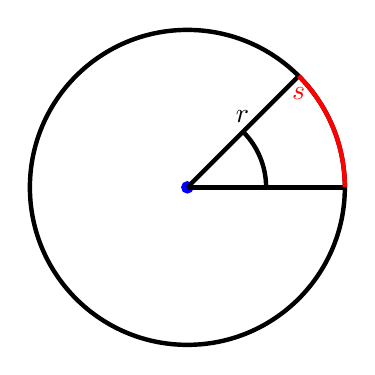
\begin{tikzpicture}
   % \draw[step=1cm,gray,very thin] (3,-3) grid (3,3);
   \filldraw[color = blue, ultra thick](0,0) circle (0.05);
    \draw[ ultra thick](0,0) circle (2);
    \draw[ultra thick] (0,0) -- (1.414,1.414);
  \node[anchor =south] at (0.7,0.7) {$r$};
    \draw[ultra thick] (0,0) -- (2,0);
    \draw[ultra thick] (1,0) arc (0:45:1) node[anchor=north]{$\uptheta$};
     \draw[ultra thick, color=red] (2,0) arc (0:45:2) node[anchor=north]{$s$};
    \end{tikzpicture}
    %}{A circle}
    \caption{A circle of radius $r$ showing how arc length around the circle corresponds to angles}
        \label{fig: radians}
\end{figure}

More generally the conversion rule is that
\begin{equation*}
\text{radians} = \frac{180^{\circ}}{\uppi}\times \text{degrees}.
\end{equation*}
The main advantage of radians comes when differentiating and expanding functions as working in degrees requires extra terms to be included and greater care to be taken. While we will not be doing any differentiation in this module we will come across some expressions where we need to work in radians for the quoted expressions to be valid. When this happens we will include a warning so that it is clear where you need to be careful.\\

One way to motivate working in radians is to think of unwinding the circle to get a straight line, for a circle of radius $r$ this length will be the circumference, if we divide this length by $r$ we will have a line if length $2\uppi$ and the angle in radians will be the distance travelled along this line. In other words, working in radians is a bit like converting from circular motion to linear motion.

\begin{figure}[ht]
    \centering
    \ThisAltText{ Another circle showing how the arc length and angle can be related to a straight line distance.}
   % \pdftooltip{
    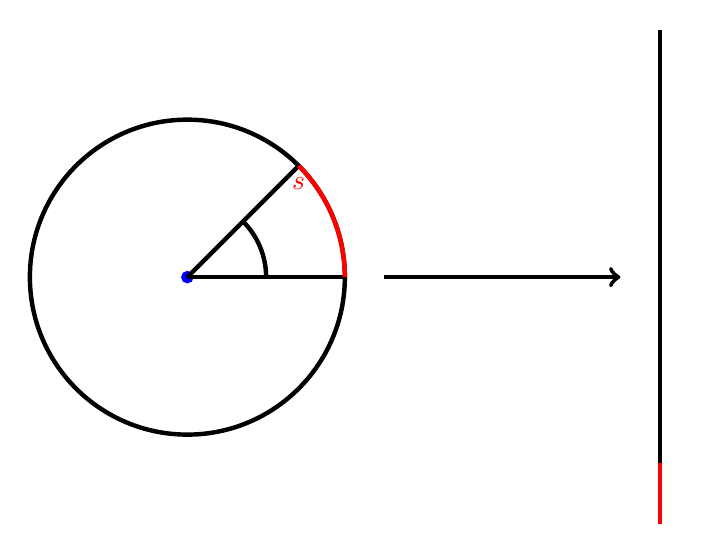
\begin{tikzpicture}
   % \draw[step=1cm,gray,very thin] (3,-3) grid (3,3);
   \filldraw[color = blue, ultra thick](0,0) circle (0.05);
    \draw[ ultra thick](0,0) circle (2);
    \draw[ultra thick] (0,0) -- (1.414,1.414);
 % \node[anchor =south] at (0.7,0.7) {$r$};
    \draw[ultra thick] (0,0) -- (2,0);
    \draw[ultra thick] (1,0) arc (0:45:1) node[anchor=north]{$\uptheta$};
     \draw[ultra thick, color=red] (2,0) arc (0:45:2) node[anchor=north]{$s$};
     \draw[ultra thick] (6,-3.14) --(6,3.14);
     \draw[ultra thick, color = red] (6,-3.14) --(6,-2.355) node[anchor=west]{$\uptheta$};
     \draw[ultra thick, ->] (2.5,0) -- (5.5,0);
    \end{tikzpicture}
   % }{A circle}
    \caption{A circle of radius $r$ showing how arc length around the circle corresponds to angles}
        \label{fig: radians 2}
\end{figure}

As evidenced in \cref{fig: radians,fig: radians 2}, it is common practice to use the Greek letter theta, $\uptheta$, to denote an angle. Other Greek letters like phi, $\upphi$ or $\upvarphi$, and psi, $\uppsi$, are sometimes used as well. It is worth spending some time familiarising yourself with these Greek letters so you do not think that they are just badly written English letters.

\section{Circular Motion}
In the second section of these notes we studied linear motion, in particular uniform motion where the acceleration is constant. In that case objects moved in straight lines. What about if an object is moving in a circle?\\

An object rotating at a steady rate is said to be in \textbf{uniform circular motion}. A good example to have in mind is a point on the perimeter of a wheel of radius $r$ rotating at a steady speed. The circumference of the wheel is $2\uppi r$ and we call the time taken for $p$ to rotate once around the wheel the \textbf{period} $T$. Another important quantity related to the period is the \textbf{frequency}, $f=1/T$ which measures the number of rotations per second. The period is measured in seconds as it is a unit of time, while the frequency is measured in Hertz or units of per second.\\

\begin{figure}[ht]
    \centering
  %  \pdftooltip{
  \ThisAltText{ A rotating wheel with a point and its instantaneous straight line velocity marked.}
    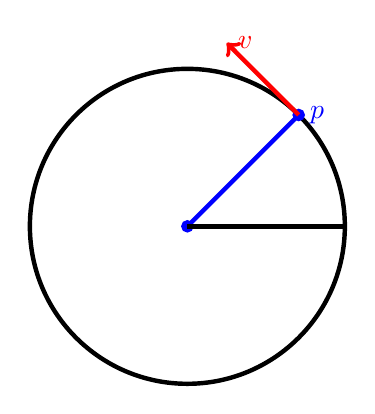
\begin{tikzpicture}
   % \draw[step=1cm,gray,very thin] (3,-3) grid (3,3);
   \filldraw[color = blue, ultra thick](0,0) circle (0.05);
    \draw[ ultra thick](0,0) circle (2);
    \draw[ultra thick, color=blue] (0,0) -- (1.414,1.414);
    \draw[ultra thick] (0,0) -- (2,0);
     \filldraw[color = blue, ultra thick](1.414,1.414) circle (0.05)node[anchor=west]{$p$};
     \draw[ultra thick, color=red, ->] (1.414,1.414)-- (0.5,2.33)node[anchor=west]{$v$};
    \end{tikzpicture}
  %  }{A rotating wheel}
    \caption{A rotating wheel with a point $p$ marked on its surface along with the instantaneous velocity of $p$.}
        \label{fig: pt on a wheel}
\end{figure}

The linear speed, or the speed if the point $p$ was moving in a straight line is 
\begin{equation*}
v=\frac{\text{circumference}}{T}=\frac{2\uppi r}{T}=2\uppi r f.
\end{equation*}
This relationship gives us away to convert between the linear motion of an object and the circular motion of its wheels.


\paragraph{Example 6.1:} A cyclist is travelling at $25\text{m/s}$ on a bicycle that has wheels of radius $750 \text{mm}$. Calculate:
\begin{itemize}
\setlength{\itemsep}{-5pt}
    \item[a)] The time for one rotation of the wheel,
    \item[b)] The rotation frequency of the wheel,
    \item[c)] The number of times the wheel rotates in a minute.
\end{itemize} 

a) Rearranging $v=2\uppi r/T$ and substituting in the numbers we have that the period is
\begin{equation*}
T=\frac{2\uppi r}{v}=2\uppi\times \frac{0.75}{25}=0.19\text{s}.
\end{equation*} 

b) The frequency is 
\begin{equation*}
f=\frac{1}{T}=\frac{1}{0.19}\text{Hz}=5.3\text{Hz}.
\end{equation*}

c) The number of rotations in a minute is then
\begin{equation*}
\text{rotations per minute} = f\times 60=320.
\end{equation*}

The angle $\uptheta$ that a rotating object moves through is called the \textbf{angular displacement}. We will almost always work with $\uptheta$ in radians, though occasionally you may see an angle quoted in degrees that you need to convert into radians. In uniform circular motion an object turns through an angle of $2\uppi/T$ radians per second, thus the angular displacement after a time $t$ is
\begin{equation}
\uptheta=\frac{2\uppi t}{T}.
\end{equation}
To understand this recall that the total distance round the circle is $2\uppi$ in radians, and $T$ is measuring the time it takes to complete a full rotation. The angular displacement is measured in radians as it is an angle. \\

The angular analogue of the speed from linear motion is the \textbf{angular speed} or angular velocity, omega  $\upomega$, which is defined as the rate of change of angular displacement and is given by
\begin{equation}
\upomega=\frac{\uptheta}{t}=\frac{2\uppi}{T}=2\uppi f.
\end{equation}
we measure angular speed in units of radians per second or $\text{rad/s}$. 

\paragraph{Example 6.2:} Consider a cyclist travelling at $ 12\text{m/s}$ on a bike with wheels of radius $0.4\text{m}$. Calculate:
\begin{itemize}
\setlength{\itemsep}{-5pt}
    \item[a)] The frequency of rotation of the wheels,
    \item[b)] The angular speed of each wheel,
    \item[c)] The angle that a wheel turns through in $0.1\text{s}$ in both radians and degrees.
\end{itemize} 

a) The circumference of a wheel is $2\uppi r=2\uppi\times 0.4 =2.5\text{m}$ and 
\begin{equation*}
T=\frac{\text{circumference}}{v}=\frac{2.5}{12}=0.21\text{s}.
\end{equation*}
The frequency is thus
\begin{equation*}
f=\frac{1}{T}=\frac{1}{0.21}=4.8\text{Hz}.
\end{equation*}

b) The angular speed is 
\begin{equation*}
\upomega=2\uppi f=30\text{rad/s}.
\end{equation*}

c) The angular displacement in $0.1\text{s}$ is
\begin{equation*}
\uptheta=\upomega t=3 \text{rad},
\end{equation*}
or in degrees this is $3\times360^{\circ}/2\uppi=170^{\circ}$.

\section{Centripetal forces}
When an object is moving in a circle at a constant speed the linear velocity is constantly changing direction. In other words the magnitude of the velocity is constant but its direction is changing. Since the objects velocity is changing in time it is accelerating. This may seem counter intuitive since we say that the motion is uniform. \\

From \cref{fig: pt on a wheel}  we see that the velocity is tangent to the circle at the objects location. As the object moves around the circle the direction of the velocity continually changes with the direction of change being towards the centre of the circle. Thus the acceleration is pointing towards the centre of the circle. This acceleration is called the \textbf{centripetal acceleration}, and is given by
\begin{equation}
a=\frac{v^{2}}{r}=\upomega^{2}r.
\label{eq: centripetal acceleration}
\end{equation}


\begin{figure}[ht]
    \centering
    \ThisAltText{ A rotating wheel with a point, its instantaneous velocity, and its centripetal acceleration marked.}
    %\pdftooltip{
    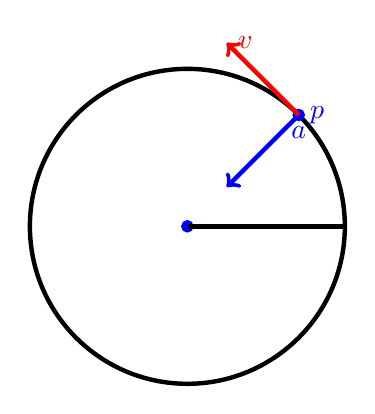
\begin{tikzpicture}
   % \draw[step=1cm,gray,very thin] (3,-3) grid (3,3);
   \filldraw[color = blue, ultra thick](0,0) circle (0.05);
    \draw[ ultra thick](0,0) circle (2);
    \draw[ultra thick, color=blue,->] (1.414,1.414)node[anchor=north]{$a$}--(0.5,0.5);
 % \node[anchor =south] at (0.7,0.7) {$r$};
    \draw[ultra thick] (0,0) -- (2,0);
  %  \draw[ultra thick] (1,0) arc (0:45:1) node[anchor=north]{$\ut$};
     %\draw[ultra thick, color=red] (2,0) arc (0:45:2) node[anchor=north]{$s$};
     \filldraw[color = blue, ultra thick](1.414,1.414) circle (0.05)node[anchor=west]{$p$};
     \draw[ultra thick, color=red, ->] (1.414,1.414)-- (0.5,2.33)node[anchor=west]{$v$};
    \end{tikzpicture}
   % }{A rotating wheel with v and a marked}
    \caption{A rotating wheel with a point $p$ marked along with its velocity and acceleration.}
        \label{fig: pt on a wheel 2}
\end{figure}


To make an object move in a circular path we need to act on it with a force that generates the inward acceleration. This resultant force is known as the \textbf{centripetal acceleration} and it acts towards the centre of the circle.\\

There are a few places where you may have come across centripetal acceleration before:
\begin{itemize}
\setlength{\itemsep}{-5pt}
    \item Satellites orbiting the earth get their centripetal force from the Earth's gravity.
    \item An object spinning round on the end of a string gets its centripetal force from the string's tension.
\end{itemize} 

For an object moving with linear velocity $v$ along a circular path of radius $r$ we know the centripetal acceleration from \cref{eq: centripetal acceleration}. By Newton's second law this corresponds to a centripetal force given by
\begin{equation}
F=m\upomega^{2}r=\frac{mv^{2}}{r}.
\label{eq: centripetal force}
\end{equation}

Note that since the centripetal force is at right angles to the direction of motion it does no work, and the kinetic energy is constant since the speed is unchanged.

%\paragraph{Example 6.3:} The wheel of the London Eye has a diameter of $130\text{m}$ and takes $30\text{min}$ for one full rotation. Calculate:
\begin{itemize}
\setlength{\itemsep}{-5pt}
    \item[a)] The speed of a capsule,
    \item[b)] The centripetal acceleration of a capsule,
    \item[c)] The centripetal force acting on a person of mass $65\text{kg}$ in a capsule.
\end{itemize} 

%a) The circumference is 
\begin{equation*}
2\uppi r=\uppi d=\uppi \times 130=408\text{m},
\end{equation*}
and the speed is 
\begin{equation*}
v=\frac{2\uppi r}{T}=\frac{408}{30\times 60}=0.23\text{m/s}.
\end{equation*}

b) The centripetal acceleration is 
\begin{equation*}
a=\frac{v^{2}}{r}=\frac{0.23^{2}}{65}=0.00079\text{m/s}^{2}=7.9\times 10^{-4}\text{m/s}^{2}.
\end{equation*}

c) The centripetal force is then 
\begin{equation*}
F=ma=65\times 7.9\times 10^{-4}=5.1\times 10^{-2}\text{N}.
\end{equation*}

%Notice that the centripetal force points inwards. Sometimes when people talk about circular motion they will mention an outward pointing centrifugal force. This is a \textbf{fictitious force} which appears if you work in the \textbf{reference frame} of the rotating object. The Coriolis force is another fictitious force that appears due to the rotation of an object. It is important to note here that fictitious does not mean that we are imagining these effects, but rather that they are not due to forces. They occur because we are in a rotating reference frame. If you go on to study more physics then you will learn more about why rotational motion results in these fictitious forces.

\section{Circular motion in action}
To finish off this section we will now discuss some concrete examples of where objects moving in circles appear in the real world:
\begin{itemize}
\setlength{\itemsep}{-5pt}
    \item Vehicles going round roundabouts.
    \item Going over hills.
    \item Banked tracks.
    \item Amusement rides
\end{itemize} 
All four of these examples are included in \citep{breithaupt2016aqa} so you can look there for further details if you want to know more.  For the case of motion on a banked track we refer the interested reader to Chapter 17.3 of \citep{breithaupt2016aqa}.

\paragraph{Going over hills.} Consider a vehicle of mass $m$ moving at speed $v$ along a road that passes over the top of a hill or a curved bridge. We will assume that the road or bridge has the shape of an arc in a circle, this may not be perfectly true but it is a good approximation and in this module we will not need to take a better approximation. The road acts on the vehicle through a support force $S$ which is opposite to the vehicle's weight $mg$. The difference between the support force and the weight acts towards the centre of the circle. This net force is a centripetal force and is given by
\begin{equation*}
mg-S=\frac{mv^{2}}{r}.
\end{equation*}
Here $r$ is the radius of curvature of the hill, in other words the radius of the circle if we pretend that the hill is part of a circle.\\

\textcolor{red}{Figures to be added to this section.}\\

If the vehicle is travelling fast enough it will lose contact with the road. This will happen for velocities higher than a critical speed $v_{0}$. When $v=v_{0}$ the support force will vanish and
\begin{equation*}
mg=\frac{mv^{2}_{0}}{r}.
\end{equation*}
As there is a factor of the mass on both sides of the equation they cancel out and we are left with the critical speed given in terms of $g$ and the radius of the circle as
\begin{equation*}
v_{0}=\pm\sqrt{gr},
\end{equation*}
the $\pm$ show that the vehicle can be heading either left or right over the hill and the condition is the same. As $g$ is approximately constant on Earth, this is essentially a geometric condition where the size of the hill determines how fast you need to go to lose contact with the road. For small hills this may not be that fast, but for a large hill you would need to go very fast.\\

If $r=5\text{m}$ then $v_{0}=\pm 7\text{m/s}$ or $15.7\text{mph}$.

\paragraph{Roundabouts.} Next consider a car of mass $m$ going in a circle round a roundabout at a speed $v$. Now the car is going round in a horizontal circle rather than a vertical circle. The centripetal force is not related to the weight of the car but rather to the sideways frictional force between the car's tires and the road,
\begin{equation*}
F_{f}=\frac{mv^{2}}{r}.
\end{equation*}
The weight of the vehicle is still important though. If the vehicle is travelling too fast, above a critical velocity $v_{0}$, then the friction will not be enough to stop the car from slipping and skidding. The limiting force is given by
\begin{equation*}
F_{0}=\frac{mv_{0}^{2}}{r}.
\end{equation*}
As $F_{0}$ is a frictional force it can be written as $F_{0}=\upmu mg$ where $\upmu$ is the \textbf{coefficient of friction}\footnote{There are actually two types of coefficients of friction: static and dynamic. In this module we do not make a distinction between them, but it is important to be aware that there is a difference as some books will use different names in different contexts.}.  Using $\upmu$ we can find an expression for $v_{0}$ analogous to that used above. The critical speed is given by
\begin{equation*}
v_{0}=\sqrt{\upmu g r},
\end{equation*}
deriving this expression is left as an exercise to the interested reader.

\paragraph{Example 6.4:} Consider a vehicle of mass $1200\text{kg}$ passing over a circular bridge whose radius of curvature is $15\text{m}$ at a speed of $10\text{m/s}$. Calculate:
\begin{itemize}
\setlength{\itemsep}{-5pt}
    \item[a)] The centripetal acceleration of the vehicle on the bridge,
    \item[b)] The support force on the vehicle when it is at the top of the bridge,
    \item[c)] The critical velocity at which the vehicle will lose contact with the road.
\end{itemize} 


a) The centripetal acceleration is found by solving 
\begin{equation*}
ma=F_{c}=\frac{mv^{2}}{r},
\end{equation*}
for $a$. In other words
\begin{equation*}
a=\frac{v^{2}}{r}=\frac{10^{2}}{15}=6.67\text{m/s}^{2}.
\end{equation*}

b) The support force is given by the difference between the cars weight and the centripetal force,
\begin{equation*}
S=mg-\frac{mv^{2}}{r}=mg-ma=m\left(g-a\right)=1200\left(9.8-6.67\right)=3756\text{N}\sim 3.8\text{kN}.
\end{equation*}

c) At the critical velocity we have that $S=0$ and $v_{0}=\sqrt{gr}$ so can just substitute the given value of $r$ into this expression to find
\begin{equation*}
v_{0}=\sqrt{gr}=\sqrt{9.8\times 15}=12.1\text{m/s}.
\end{equation*}


\paragraph{Amusement rides.} Consider the sort of rides that you may find at a fairground or at a theme park. Many of these involve circular motion in some way. The prime example would be a Ferris wheel or a big sightseeing wheel like the London Eye.\\

Examples of these sort of rides include: 

\begin{itemize}
\setlength{\itemsep}{-5pt}
    \item The Big Dipper: You are taken at high speed through a big dip and feel pushed up out of your seat. This is essentially the opposite of crossing the top of a hill, with the support force now acting upwards, since that is towards the centre of the circle. At the bottom of the dip the difference between $S$ and the weight again gives the centripetal force and from that we can determine the velocity:
    \begin{equation*}
    S-mg=\frac{mv^{2}}{r}.
    \end{equation*}
    \item A very long swing: Imagine a person of mass $m$ on a very long swing of length $L$ released from a height of $h$ above the ground. At the start of the swing all of the energy is potential energy $E_{P}=mgh$ at the bottom of the swing all of the energy is kinetic $E_{K}=\frac{1}{2}mv^{2}$. This is when the swing passes through equilibrium. The speed is maximum when the swing is going through equilibrium and the kinetic energy is equal to the initial potential energy:
    \begin{equation*}
    \frac{1}{2}mv^{2}=E_{K}=E_{P}=mgh.
    \end{equation*}
This leads to $v=\sqrt{2gh}$.
If $h=L$, so that the swing touches the ground at the bottom then the centripetal force is
\begin{equation*}
S-mg=\frac{mv^{2}}{L}=\frac{2mgh}{L}=2mg,
\end{equation*}
so $S=3mg$.
\item The Big Wheel: Consider a big wheel, sometimes called a \textbf{Gravitron}, which takes passengers around in a vertical circle on the inside of the circumference of the circle. The wheel needs to turn fast enough to stop the passengers falling out. When the passenger is at the top of the circle the reaction force $R$ acts downwards parallel to the weight such that the resultant force is $R+mg$. This resultant force is a centripetal force which determines the velocity necessary so that the passengers stick to the outside:
\begin{equation*}
mg+R=\frac{mv^{2}}{r}.
\end{equation*}
At a particular speed $v_{0}^{2}=gr$ the reaction force vanishes, $R=0$. This makes the person feel weightless.
\end{itemize} 


\paragraph{Example 6.5:} Consider a very long swing with length $L=32\text{m}$. A person of mass $m=69\text{kg}$ is on the swing and descends from a position where the swing is horizontal. Calculate:
\begin{itemize}
\setlength{\itemsep}{-5pt}
    \item[a)] The speed of the person at the lowest point,
    \item[b)] The centripetal acceleration at the lowest point,
    \item[c)] The support force on the person at the lowest point.
\end{itemize} 

a) We are starting from $90^{\circ}$ so can take $h=L=32\text{m}$. Thus the speed at the lowest point is 
\begin{equation*}
v=\sqrt{2gh}=\sqrt{2\times 9.8\times 32}=25\text{m/s}.
\end{equation*}

b) The centripetal acceleration is 
\begin{equation*}
a=\frac{v^{2}}{L}=\frac{25^{2}}{32}=19.6\text{m/s}^{2},
\end{equation*}
this is also twice the acceleration due to gravity or $2g$.

c) The support force at the lowest point is given by 
\begin{equation*}
S=mg+\frac{2mgh}{L}=3mg=3\times 9.8\times 69=2030\text{N}.
\end{equation*}

The basic ideas of circular motion that we have seen here are also useful in situations that may at first appear to have nothing to do with moving in a circle. In the next section we will study oscillating objects like springs and pendulums and find the hidden circles that helps us to describe their motion.